% presentaciones/sesion09-cap09/sesion09.tex
% Sesión 9 — Capítulo 9: Base tecnológica para el análisis del recorrido
% Laboratorio: Gestión de datos, comportamiento y perfiles del consumidor digital
% Lic. en Mercadotecnia Digital · ESCA Unidad Santo Tomás · IPN
% Fuente de contenido: libro-consumidor-digital/partes/parte2/cap09.tex
% Figuras reutilizadas del libro (TikZ y MATLAB) sin copiarlas: ver \graphicspath y \input.
\documentclass[aspectratio=169,xcolor=dvipsnames]{beamer}
\usetheme{Berlin}

%----------------------------------------------------------------------------------------
%   PALETA INSTITUCIONAL IPN (Manual de Identidad Gráfica, Pantone 222C)
%----------------------------------------------------------------------------------------
\usepackage[dvipsnames,svgnames,x11names]{xcolor}
\definecolor{IPNguinda}{HTML}{6F1D46}       % Pantone 222C oficial — color primario
\definecolor{IPNguindaOsc}{HTML}{45102C}    % sombra / paleta secundaria
\definecolor{IPNguindaClara}{HTML}{F4E9EF}  % fondo de bloques normales
\definecolor{IPNdorado}{HTML}{B8975A}       % dorado — SOLO enlaces y detalles del cierre
\definecolor{IPNterracota}{HTML}{9C5B44}    % alertblock
\definecolor{IPNterracotaClara}{HTML}{F6ECE6}
\definecolor{IPNbronce}{HTML}{8C6B3F}       % exampleblock
\definecolor{IPNbronceClaro}{HTML}{F5F0E3}
\definecolor{IPNgris}{HTML}{58595B}         % texto secundario / notas

% Alias con los nombres de config/colores.tex del libro, para que las figuras
% TikZ del libro se puedan \input sin modificarlas
\colorlet{guindaIPN}{IPNguinda}
\colorlet{guindaIPNOsc}{IPNguindaOsc}
\colorlet{guindaIPNClara}{IPNguindaClara}
\colorlet{doradoIPN}{IPNdorado}
\colorlet{bronceIPN}{IPNbronce}
\colorlet{bronceIPNClaro}{IPNbronceClaro}
\colorlet{grisIPN}{IPNgris}
\colorlet{terracotaIPN}{IPNterracota}
\colorlet{terracotaIPNClara}{IPNterracotaClara}
\definecolor{colorLaboratorio}{HTML}{1B6E7A}

\setbeamercolor{palette primary}{bg=IPNguinda,fg=white}
\setbeamercolor{palette secondary}{bg=IPNguindaOsc,fg=white}
\setbeamercolor{palette tertiary}{bg=IPNguindaOsc,fg=white}
\setbeamercolor{palette quaternary}{bg=IPNguinda,fg=white}
\setbeamercolor{structure}{fg=IPNguinda}
\setbeamercolor{title}{bg=IPNguinda,fg=white}
\setbeamercolor{frametitle}{bg=IPNguinda,fg=white}
\setbeamercolor{block title}{bg=IPNguinda,fg=white}
\setbeamercolor{block body}{bg=IPNguindaClara,fg=black}
\setbeamercolor{block title alerted}{bg=IPNterracota,fg=white}
\setbeamercolor{block body alerted}{bg=IPNterracotaClara,fg=black}
\setbeamercolor{block title example}{bg=IPNbronce,fg=white}
\setbeamercolor{block body example}{bg=IPNbronceClaro,fg=black}
\setbeamercolor{alerted text}{fg=IPNterracota}
\setbeamercolor{item}{fg=IPNguinda}
\setbeamercolor{section in toc}{fg=IPNguinda}
\setbeamercolor{footline}{bg=IPNguindaOsc,fg=white}

\usepackage[spanish,es-noshorthands,es-nodecimaldot]{babel}
\usepackage{csquotes}
\usepackage{hyperref}
\usepackage{graphicx}
\usepackage{booktabs}
\usepackage{array}
\usepackage{amsmath}
\setbeamertemplate{caption}[numbered]
\usepackage{xurl}
\usepackage{adjustbox}
\usepackage{tikz}
\usetikzlibrary{arrows.meta,positioning,shapes.geometric}
\usepackage{pgfplots}
\pgfplotsset{compat=1.18}

\graphicspath{{Figures/}{../../libro-consumidor-digital/figuras/matlab/}}
\newcommand{\figtikz}[1]{../../libro-consumidor-digital/figuras/tikz/#1}
\newcommand{\fuente}[1]{{\tiny\color{IPNgris}Fuente: #1}}

\hypersetup{
    colorlinks=true,
    linkcolor=IPNdorado,
    filecolor=IPNguinda,
    urlcolor=IPNguinda,
    citecolor=IPNguinda,
    pdftitle={Sesion 9 - Base tecnologica del recorrido},
    pdfauthor={Dr. Aboud Barsekh-Onji},
}

%----------------------------------------------------------------------------------------
%   CODE LISTINGS — sintaxis ESTÁNDAR del lenguaje
%----------------------------------------------------------------------------------------
\usepackage{listings}
\definecolor{backcolour}{rgb}{0.97,0.97,0.99}
\definecolor{codegreen}{rgb}{0,0.6,0}

\lstdefinestyle{MATLABStyle}{
  language=Matlab,
  basicstyle=\ttfamily\scriptsize,
  keywordstyle=\color{blue}\bfseries,
  commentstyle=\color{codegreen},
  stringstyle=\color{violet},
  breaklines=true,
  numbers=left,
  numbersep=5pt,
  frame=lines,
  backgroundcolor=\color{backcolour}
}
\lstset{style=MATLABStyle}

%----------------------------------------------------------------------------------------
%   TITLE CONFIGURATION
%----------------------------------------------------------------------------------------
\logo{
\includegraphics[height=0.75cm]{ipn-escudo.png}}
\title[Sesión 9 · Base tecnológica del recorrido]{Base tecnológica para el análisis del recorrido}
\subtitle{Sesión 9 · Unidad II — Capítulo 9}
\author{Dr. Aboud Barsekh-Onji}
\institute[IPN]{
    Instituto Politécnico Nacional \\
    \small ESCA Unidad Santo Tomás · Lic. en Mercadotecnia Digital \\
    \footnotesize Laboratorio: Gestión de datos, comportamiento y perfiles del consumidor digital
}
\date{\today}

%----------------------------------------------------------------------------------------
%   AUTO AGENDA AT EACH SECTION
%----------------------------------------------------------------------------------------
\AtBeginSection[]{
  \begin{frame}{Agenda}
    \tableofcontents[currentsection]
  \end{frame}
}



\begin{document}

\begin{frame}
    \titlepage
    \vspace{-4pt}
    \begin{center}
        {\tiny\color{IPNgris} ORCID: \href{https://orcid.org/0009-0004-5440-8092}{0009-0004-5440-8092}}
    \end{center}
\end{frame}

%------------------------------------------------
\section{Encuadre}
%------------------------------------------------

\begin{frame}{Ficha de la sesión}
\begin{columns}[T]
  \column{0.52\textwidth}
  \begin{block}{Unidad II}
    \small Proceso de toma de decisión de compra digital
  \end{block}
  \begin{block}{Tema del programa (2.4 Base tecnológica)}
    \scriptsize
    \begin{itemize}
      \item[2.4.1] Temas selectos de buscadores y plataformas de gestión integral, redes sociales y comercio electrónico
    \end{itemize}
  \end{block}
  \column{0.44\textwidth}
  \begin{block}{Carga horaria}
    \small Teoría 3.0 h · Práctica 2.0 h\\ Aprendizaje autónomo 1.0 h
  \end{block}
  \begin{exampleblock}{Competencia de la unidad}
    \small Examina el proceso de toma de decisiones de compra del consumidor digital a partir de su recorrido y figuras participantes.
  \end{exampleblock}
\end{columns}
\end{frame}

\begin{frame}{Al terminar la sesión podrás\ldots}
\begin{enumerate}
  \item \textbf{Ubicar} cuatro categorías de herramienta en las capas de captura, identidad, análisis y activación.
  \vspace{4pt}
  \item \textbf{Evaluar} una herramienta con criterios durables, sin depender de una marca.
  \vspace{4pt}
  \item \textbf{Obtener} pesos de criterios con AHP y comprobar si tus juicios son consistentes.
  \vspace{4pt}
  \item \textbf{Ordenar} alternativas con TOPSIS y localizar el peso en que cambia la elección.
\end{enumerate}
\vspace{6pt}
\begin{alertblock}{Recordatorio}
  Aprendizaje autónomo de la Sesión 8: entrega en la fecha acordada en clase, en su carpeta del portafolio. \textbf{Hoy se cierra el entregable único} de la práctica «Recorrido del consumidor digital».
\end{alertblock}
\end{frame}

\begin{frame}{Arranque: ¿con qué se mide tu negocio?}
\begin{columns}[T]
  \column{0.55\textwidth}
  \begin{exampleblock}{Pregunta de arranque}
    Si tuvieran que \textbf{medir el recorrido} del caso de su equipo, ¿qué herramienta usarían? ¿Por qué esa y no otra?\\[4pt]
    ¿Qué \textbf{dato de las personas} se llevaría?
  \end{exampleblock}
  \vspace{4pt}
  {\small\color{IPNgris} Puente con las Sesiones 6 a 8: el caso del equipo ya tiene proceso, recorrido y figuras.}
  \column{0.41\textwidth}
  \begin{block}{Dinámica (10 min)}
    \small
    \begin{enumerate}
      \item Equipos: nombren la herramienta y tres razones (3 min).
      \item Pizarrón: ¿cuántas razones son \textbf{de costo} y cuántas de \textbf{privacidad o datos}?
    \end{enumerate}
  \end{block}
\end{columns}
\end{frame}

%------------------------------------------------
\section[Apertura]{Caso de apertura}
%------------------------------------------------

\begin{frame}{Dos historias, una moraleja}
\begin{columns}[T]
  \column{0.48\textwidth}
  \begin{block}{Hecho documentado (octubre de 2026)}
    \small Universal Analytics \textbf{dejó de procesar datos el 1 de julio de 2023}; el 1 de julio de 2024 se perdió el acceso a su interfaz y a su API (Google, 2026). Quien no exportó, \textbf{perdió el histórico}.
  \end{block}
  \column{0.48\textwidth}
  \begin{exampleblock}{Caso ficticio}
    \small Una tienda contrata \textbf{grabación de sesiones}. Siete meses después descubre que \textbf{también grabó lo que escribían en el formulario de pago}, sin consentimiento específico y sin forma fácil de exportar y borrar.
  \end{exampleblock}
\end{columns}
\vspace{6pt}
\begin{alertblock}{La moraleja}
  Elegir la herramienta que analiza el recorrido es una decisión con costos de \textbf{privacidad, interoperabilidad y dinero} que se pagan después. Por eso hoy: \textbf{criterios y método}, no catálogo de marcas.
\end{alertblock}
\end{frame}

%------------------------------------------------
\section[Capas]{2.4.1 Cuatro capas, cuatro categorías}
%------------------------------------------------

\begin{frame}{El dato del recorrido pasa por cuatro capas}
\begin{center}
  \adjustbox{max width=0.97\linewidth,max height=0.6\textheight}{\input{\figtikz{cap09-pila-analitica}}}
\end{center}
\vspace{-2pt}
{\scriptsize Se \textbf{captura}, se \textbf{asocia a una identidad}, se \textbf{analiza} y se \textbf{activa}. Cada categoría de herramienta opera sobre una o varias capas.}
\fuente{elaboración propia.}
\end{frame}

\begin{frame}{Mapas de calor y grabación de sesiones}
\begin{columns}[T]
  \column{0.46\textwidth}
  \begin{block}{Dos tipos de análisis}
    \small \textbf{Agregado}: dónde da clic la mayoría. \textbf{Cualitativo individual}: reproduce la sesión de una persona.
  \end{block}
  \column{0.50\textwidth}
  \begin{exampleblock}{Tres criterios para cualquier herramienta}
    \scriptsize
    \begin{enumerate}
      \item \textbf{Cobertura} de eventos capturados.
      \item \textbf{Privacidad y consentimiento} en la captura (LFPDPPP vigente).
      \item Vincular el clic con la \textbf{etapa del recorrido}, no solo con la página.
    \end{enumerate}
  \end{exampleblock}
\end{columns}
\vspace{4pt}
\begin{alertblock}{Riesgo típico}
  \small Capturar \textbf{campos sensibles} (pagos, contraseñas, salud) por no haber configurado exclusiones.
\end{alertblock}
\end{frame}

\begin{frame}{Analítica de embudo y atribución}
\begin{columns}[T]
  \column{0.50\textwidth}
  \begin{block}{Un embudo útil}
    \small Sus etapas reflejan \textbf{intención real}, no solo eventos técnicos («vista de página»). Mide el \textbf{abandono etapa por etapa}. Instrumenta las etapas AIDAS: \textbf{no las sustituye}.
  \end{block}
  \column{0.46\textwidth}
  \begin{alertblock}{Atribución}
    \small Si solo ofrece \textbf{último clic}, repite el error del laboratorio de la Sesión 7 (Anderl et al., 2016): el canal que abre no recibe crédito.
  \end{alertblock}
\end{columns}
\vspace{6pt}
{\small\color{IPNgris} El capítulo 5 (Google Analytics 4) muestra un embudo y una exploración en una herramienta concreta, y cuándo se pueden exportar los datos.}
\end{frame}

\begin{frame}{Plataformas de datos de clientes (CDP)}
\begin{columns}[T]
  \column{0.50\textwidth}
  \begin{block}{Definición de referencia (Gartner, 2026)}
    \small Aplicación que \textbf{unifica y gestiona datos de clientes} de múltiples fuentes y crea \textbf{perfiles persistentes y gobernados} para análisis, decisión y activación.
  \end{block}
  \column{0.46\textwidth}
  \begin{exampleblock}{Cuatro criterios durables}
    \scriptsize
    \begin{enumerate}
      \item Identidad entre dispositivos: ¿\textbf{real o probabilística}?
      \item \textbf{Gobernanza y consentimiento}.
      \item Activación \textbf{en tiempo real} o solo reportes.
      \item Grado de \textbf{agentes de IA} que activan solos.
    \end{enumerate}
  \end{exampleblock}
\end{columns}
\end{frame}

\begin{frame}{Frontera (vigente a octubre de 2026): dos rutas para las CDP}
\begin{columns}[T]
  \column{0.48\textwidth}
  \begin{block}{\textit{Platformization}}
    \small La CDP se vuelve una \textbf{plataforma general de datos}.
  \end{block}
  \column{0.48\textwidth}
  \begin{block}{\textit{Agentification}}
    \small La CDP incorpora \textbf{agentes de IA} que activan de forma autónoma.
  \end{block}
\end{columns}
\vspace{6pt}
\begin{alertblock}{Cómo leerlo}
  \small Es una lectura de una firma de analistas (Gartner, 2026): útil para ver la categoría, \textbf{no una fuente académica}, y probablemente cambie. El criterio que sobrevive: \textbf{si una herramienta activa sola, ¿quién responde por la decisión?}
\end{alertblock}
\end{frame}

\begin{frame}{Redes sociales y comercio electrónico: tres preguntas}
\begin{columns}[T]
  \column{0.31\textwidth}
  \begin{block}{Cobertura omnicanal}
    \small ¿Cubre redes, sitio propio y mercado en línea con una identidad común? (Verhoef et al., 2015.)
  \end{block}
  \column{0.31\textwidth}
  \begin{exampleblock}{Atribución multi-touch}
    \small ¿Se puede ver \textbf{qué canal ayudó}, no solo el último clic?
  \end{exampleblock}
  \column{0.31\textwidth}
  \begin{block}{Integración}
    \small ¿Se conecta con la analítica de embudo y la CDP?
  \end{block}
\end{columns}
\vspace{6pt}
\begin{alertblock}{Ninguna pregunta menciona una marca}
  \small Las tres \textbf{sobreviven} a la suite que hoy domina.
\end{alertblock}
\end{frame}

\begin{frame}{Cuatro categorías, un criterio principal cada una}
\scriptsize
\begin{center}
\begin{tabular}{@{}>{\raggedright}p{2.5cm}>{\raggedright}p{2.7cm}>{\raggedright}p{3.2cm}>{\raggedright\arraybackslash}p{2.4cm}@{}}
\toprule
\textbf{Categoría} & \textbf{Responde a} & \textbf{Criterio durable} & \textbf{Riesgo regulatorio} \\
\midrule
Mapas de calor y sesiones & ¿Dónde se atoran? & Vinculación con la etapa; exclusión de campos sensibles & Datos personales sin consentimiento \\
Embudo y atribución & ¿En qué etapa se pierden y qué canal ayuda? & Etapas con intención; multi-touch & Identificadores y consentimiento \\
CDP & ¿Quién es esta persona entre canales? & Identidad real; gobernanza & Perfilamiento y cruce de fuentes \\
Suites de redes y comercio & ¿Cómo coordino los canales? & Omnicanal; integración & Publicidad a menores, transparencia \\
\bottomrule
\end{tabular}
\end{center}
\fuente{elaboración propia con base en Gartner (2026) y Verhoef et al. (2015).}
\end{frame}

%------------------------------------------------
\section[Evidencia]{Evidencia: qué sí y qué no se reporta}
%------------------------------------------------

\begin{frame}{Lo que se mide y lo que no se afirma}
\begin{columns}[T]
  \column{0.50\textwidth}
  \begin{block}{Lo que sí}
    \small \textbf{104.9 millones} de personas de 6 años o más usaron internet en México en 2025 (INEGI, 2026). Cada una deja rastros que alguna capa puede capturar y \textbf{cada captura exige base legal} (LFPDPPP).
  \end{block}
  \column{0.46\textwidth}
  \begin{alertblock}{Lo que no}
    \small \textbf{Ninguna cuota de mercado} de herramientas: las cifras vienen de blogs de proveedores y analistas, no de fuentes primarias verificables. Lo verificable es la \textbf{estructura} de criterios.
  \end{alertblock}
\end{columns}
\fuente{INEGI (2026), ENDUTIH 2025; Asociación Mexicana de Venta Online (2026).}
\end{frame}

%------------------------------------------------
\section[Método]{De criterios a decisión: AHP y TOPSIS}
%------------------------------------------------

\begin{frame}{Los criterios no deciden por sí solos}
\begin{center}
  \adjustbox{max width=0.9\linewidth,max height=0.52\textheight}{\input{\figtikz{cap09-ahp-topsis}}}
\end{center}
\vspace{-2pt}
\begin{itemize}
  \scriptsize
  \item \textbf{AHP} (Saaty, 1977): en vez de pedir pesos, pide \textbf{comparaciones por pares} y de ellas obtiene los pesos.
  \item \textbf{TOPSIS} (Hwang y Yoon, 1981): ordena por \textbf{cercanía a la solución ideal} y lejanía de la peor.
\end{itemize}
\fuente{elaboración propia con base en Saaty (1977) y Hwang y Yoon (1981).}
\end{frame}

%------------------------------------------------
\section[Laboratorio]{Laboratorio MATLAB}
%------------------------------------------------

\begin{frame}{Laboratorio: elegir una herramienta con AHP y TOPSIS}
\begin{block}{Objetivo}
  Obtener los pesos de cuatro criterios con AHP, verificar su consistencia, ordenar cinco \textbf{tipos} de herramienta con TOPSIS y localizar el peso del costo en que cambia la elección.
\end{block}
\begin{columns}[T]
  \column{0.50\textwidth}
  \begin{exampleblock}{AHP}
    \scriptsize
    Matriz $A$ con $a_{ij}$ = cuántas veces importa más $i$ que $j$; $a_{ji}=1/a_{ij}$. Pesos = vector propio principal.
    \[ \mathrm{CR}=\frac{\lambda_{\max}-n}{(n-1)\,\mathrm{RI}} < 0.10 \]
  \end{exampleblock}
  \column{0.46\textwidth}
  \begin{block}{TOPSIS}
    \scriptsize
    Normaliza, pondera y mide $d^{+}$ (a la ideal) y $d^{-}$ (a la peor):
    \[ C_i=\frac{d_i^{-}}{d_i^{+}+d_i^{-}} \]
    En el costo, \textbf{menos es mejor}.
  \end{block}
\end{columns}
\end{frame}

\begin{frame}[fragile]{El script: \texttt{cap09\_seleccion\_plataforma.m}}
\begin{columns}[T]
  \column{0.62\textwidth}
\begin{lstlisting}[basicstyle=\ttfamily\tiny]
%% ==================================
%  PARAMETROS: UNICA SECCION QUE
%  EL ESTUDIANTE DEBE EDITAR
%  ==================================
cobVsPriv = 2;      % cobertura / privacidad
cobVsInterop = 3;   % cobertura / interoper.
cobVsCosto = 3;     % cobertura / costo
privVsInterop = 2;  % privacidad / interoper.
privVsCosto = 2;    % privacidad / costo
interopVsCosto = 1; % interoper. / costo
% Escala de Saaty: 1 igual, 3, 5, 7, 9
% 1/3 = 0.333 invierte la comparacion
\end{lstlisting}
  \column{0.34\textwidth}
  \begin{block}{Reglas y rangos}
    \scriptsize
    \begin{itemize}
      \item Cada juicio: real entre \textbf{1/9 y 9}.
      \item \textbf{Cinco tipos genéricos} de herramienta con calificaciones \textbf{sintéticas}; no se evalúa ninguna marca.
      \item Sin azar.
    \end{itemize}
  \end{block}
  \begin{exampleblock}{Sin MATLAB}
    \scriptsize \texttt{cap09\_seleccion\_\allowbreak plataforma\_interactivo.html}: mismos juicios y casos A, B, C.
  \end{exampleblock}
\end{columns}
\end{frame}

\begin{frame}{Salida: pesos AHP y cercanía TOPSIS}
\begin{center}
  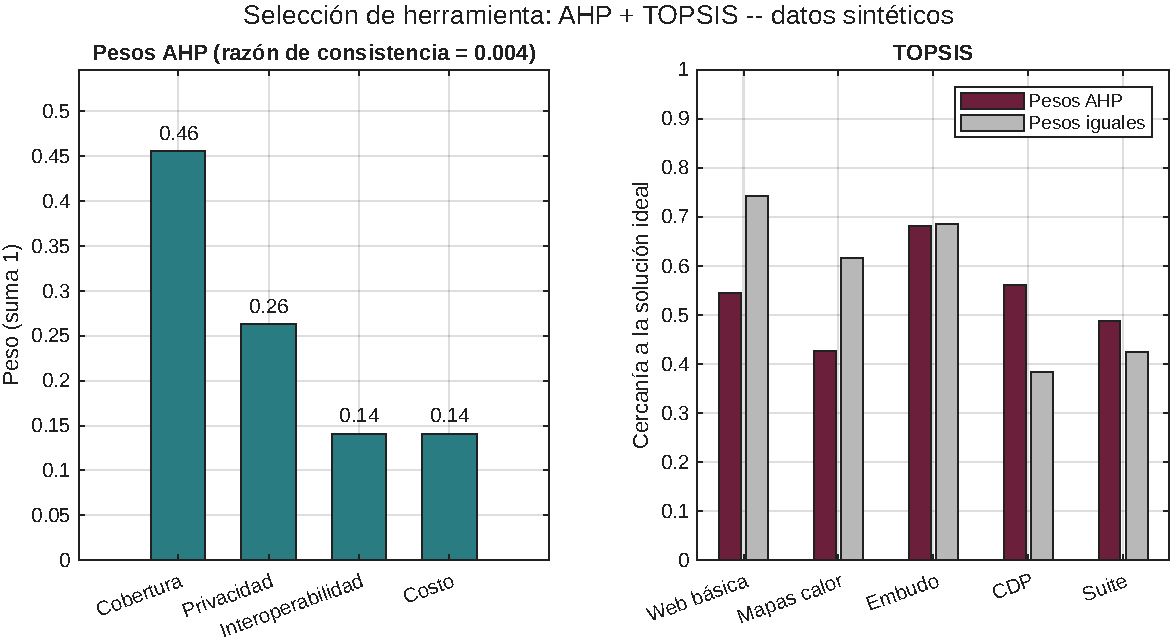
\includegraphics[width=\linewidth,height=0.62\textheight,keepaspectratio]{cap09_ahp_topsis.pdf}
\end{center}
\vspace{-4pt}
\begin{center}
  \small Pesos: 0.455 / 0.263 / 0.141 / 0.141 · razón de consistencia \textbf{0.004} · elige \textbf{analítica de embudo}; con pesos iguales, \textbf{analítica web básica}
\end{center}
\fuente{elaboración propia, MATLAB, datos sintéticos.}
\end{frame}

\begin{frame}{Interpretación: los juicios cambian la elección}
\begin{columns}[c]
  \column{0.48\textwidth}
  \begin{block}{Lo que muestra la figura}
    \small Con los juicios de AHP gana el embudo; con pesos iguales, la herramienta básica. \textbf{Qué importa más cambia la elección}.
  \end{block}
  \begin{alertblock}{Recomendación de método}
    \small Que \textbf{cada integrante} haga sus juicios por separado y se \textbf{discutan las diferencias}.
  \end{alertblock}
  \column{0.48\textwidth}
  \begin{exampleblock}{AHP no elimina la subjetividad}
    \small La \textbf{hace visible}: los juicios quedan escritos, se pueden comparar y se puede medir si se contradicen.
  \end{exampleblock}
\end{columns}
\end{frame}

\begin{frame}{Salida: ¿cuándo cambia la herramienta elegida?}
\begin{center}
  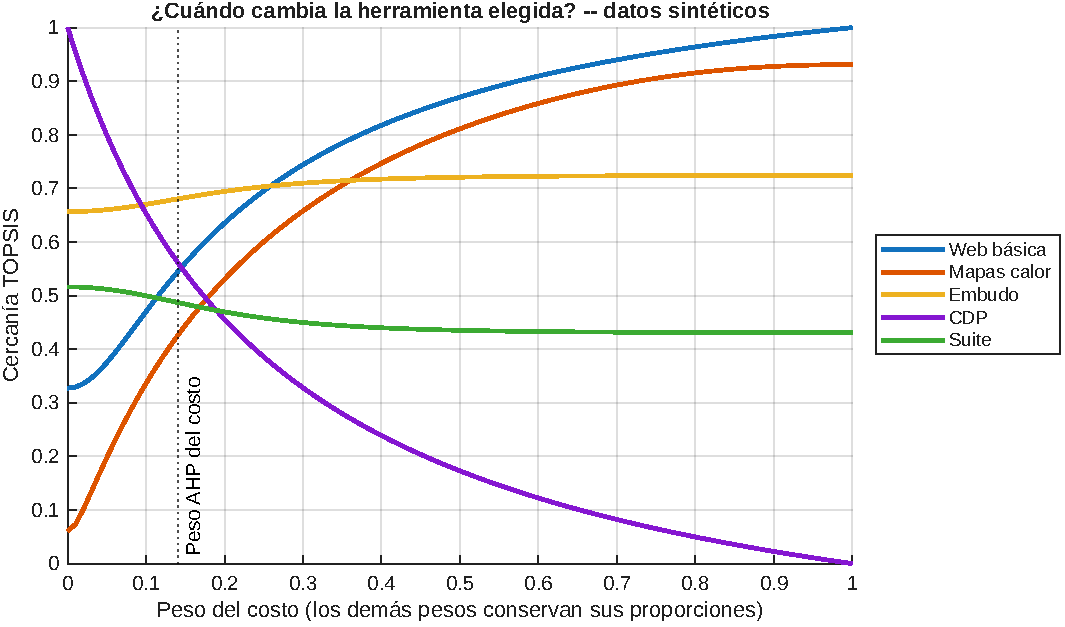
\includegraphics[width=\linewidth,height=0.62\textheight,keepaspectratio]{cap09_sensibilidad_costo.pdf}
\end{center}
\vspace{-4pt}
\begin{center}
  \small Costo $<$0.09: plataforma de datos · 0.10 a 0.25: embudo · $\geq$0.26: herramienta básica
\end{center}
\fuente{elaboración propia, MATLAB, datos sintéticos.}
\end{frame}

\begin{frame}{Interpretación: un intervalo, no un ganador único}
\begin{columns}[c]
  \column{0.48\textwidth}
  \begin{block}{Lo que enseña}
    \small La decisión no es un número: es \textbf{un intervalo de pesos} en que cada alternativa gana. Comunicarlo así es \textbf{más honesto} que reportar un solo ganador.
  \end{block}
  \column{0.48\textwidth}
  \begin{alertblock}{Aplicado al equipo}
    \small Si su peso de costo cae cerca de un cambio de ganador, \textbf{la recomendación es frágil}: dígalo.
  \end{alertblock}
\end{columns}
\end{frame}

\begin{frame}{Ejercicio propuesto: tres corridas}
\begin{columns}[T]
  \column{0.55\textwidth}
  \begin{exampleblock}{Casos (solo el bloque de parámetros)}
    \scriptsize
    \begin{itemize}
      \item[\textbf{A}] Valores por defecto.
      \item[\textbf{B}] \textbf{El costo manda}: 0.333 / 0.5 / 0.2 / 1 / 0.5 / 0.333.
      \item[\textbf{C}] \textbf{Juicios contradictorios}: 5 / 0.333 / 3 / 0.2 / 3 / 7.
    \end{itemize}
  \end{exampleblock}
  \column{0.41\textwidth}
  \scriptsize
  \begin{tabular}{@{}lccc@{}}
    \toprule
    Caso & Peso máx. & CR & Elige \\
    \midrule
    A & \rule{0.8cm}{0.4pt} & \rule{0.8cm}{0.4pt} & \rule{0.8cm}{0.4pt} \\[2pt]
    B & \rule{0.8cm}{0.4pt} & \rule{0.8cm}{0.4pt} & \rule{0.8cm}{0.4pt} \\[2pt]
    C & \rule{0.8cm}{0.4pt} & \rule{0.8cm}{0.4pt} & \rule{0.8cm}{0.4pt} \\
    \bottomrule
  \end{tabular}\\[2pt]
  {\tiny CR: razón de consistencia. Peso máx.: el mayor de los cuatro pesos y su criterio.}
\end{columns}
\vspace{2pt}
\begin{block}{Respondan con sus corridas}
  \scriptsize
  \begin{enumerate}
    \item Caso B: ¿qué peso domina y qué herramienta gana?
    \item Caso C: ¿qué dice la razón de consistencia y qué deben hacer antes de confiar en la elección?
    \item ¿Por qué un método multicriterio no elimina la subjetividad sino que la hace visible?
  \end{enumerate}
\end{block}
\end{frame}

\begin{frame}{Cierre del entregable único: «Recorrido del consumidor digital»}
\begin{columns}[T]
  \column{0.52\textwidth}
  \begin{block}{Qué integra (15 h, cuatro sesiones)}
    \scriptsize
    \begin{enumerate}
      \item Caso real y sus \textbf{cinco etapas} (S6).
      \item \textbf{Mapa} del recorrido e \textbf{infografía} de figuras (S6, S7).
      \item Los \textbf{cuatro cuadros} de casos A, B y C.
      \item \textbf{Aplicación de criterios} a dos herramientas reales (S9).
      \item \textbf{Conclusión propia} de una cuartilla.
    \end{enumerate}
  \end{block}
  \column{0.44\textwidth}
  \begin{alertblock}{La pregunta de la conclusión}
    \small ¿Qué \textbf{decisión de mercadotecnia} cambiaría el análisis del caso, y \textbf{con qué límites}? Usen al menos un resultado de cada laboratorio.
  \end{alertblock}
\end{columns}
\end{frame}

\begin{frame}{Práctica con sus propios datos: app HTML}
\begin{columns}[T]
  \column{0.54\textwidth}
  \begin{block}{\texttt{cap09\_seleccion\_datos\_propios.html}}
    \small Sin MATLAB y sin conexión: suban un Excel con \textbf{sus datos} y recorran 5 pasos:
    \scriptsize
    \begin{enumerate}
      \item Su matriz de decisión.
      \item AHP: de los juicios a los pesos y su consistencia.
      \item TOPSIS: ordenar las alternativas.
      \item Sensibilidad al peso de un criterio.
      \item Lectura de negocio y descarga en Excel.
    \end{enumerate}
  \end{block}
  \column{0.42\textwidth}
  \begin{exampleblock}{Reglas del archivo}
    \scriptsize
    \begin{itemize}
      \item Hoja \texttt{Alternativas}: nombres y de 2 a 8 criterios.
      \item Hojas \texttt{Criterios} y \texttt{Juicios} (opcionales): lista o matriz.
      \item \textbf{Sin} datos personales: nombres de herramientas o proveedores.
      \item Sus datos \textbf{no salen} de su computadora.
    \end{itemize}
  \end{exampleblock}
\end{columns}
\end{frame}

\begin{frame}{Ética: elegir herramienta es decidir sobre datos de terceros}
\begin{alertblock}{La herramienta recoge datos de personas que no participaron en la decisión}
  Una herramienta barata y eficaz que \textbf{viola la privacidad} no es una herramienta barata.
\end{alertblock}
\begin{block}{Tres reglas prácticas}
  \begin{itemize}
    \item \textbf{Minimización:} capturar solo lo que la pregunta exige y excluir campos sensibles.
    \item \textbf{Consentimiento específico:} avisar y obtener consentimiento antes de grabar sesiones; verificar la LFPDPPP \textbf{vigente al implementar}.
    \item \textbf{Salida:} elegir herramientas que permitan \textbf{exportar y borrar} los datos de una persona.
  \end{itemize}
\end{block}
\end{frame}

%------------------------------------------------
\section[Caso]{Estudio de caso}
%------------------------------------------------

\begin{frame}{Caso: tres personas, tres prioridades}
\begin{exampleblock}{Caso ficticio}
  Tres personas de una agencia deben elegir una herramienta para analizar el recorrido de una marca de ropa en línea.
\end{exampleblock}
\begin{columns}[T]
  \column{0.31\textwidth}
  \begin{block}{Finanzas}
    \small El \textbf{costo} es \enquote{muchísimo más importante} que el resto.
  \end{block}
  \column{0.31\textwidth}
  \begin{block}{Datos}
    \small Prioriza la \textbf{cobertura} del recorrido.
  \end{block}
  \column{0.31\textwidth}
  \begin{block}{Legal}
    \small Exige que \textbf{privacidad y consentimiento} pesen más que todo.
  \end{block}
\end{columns}
\vspace{4pt}
\begin{alertblock}{El grupo}
  \small Cada una llena su matriz por separado. Al promediar, la razón de consistencia del grupo es \textbf{0.17}.
\end{alertblock}
\end{frame}

\begin{frame}{Preguntas guía}
\small
\begin{enumerate}
  \item ¿Qué indica una \textbf{razón de consistencia de 0.17} y qué debería hacer el grupo antes de continuar?
  \vspace{3pt}
  \item Propongan cómo \textbf{reconciliar los tres juicios}: promedio, discusión o consenso con rangos. Justifiquen.
  \vspace{3pt}
  \item ¿Qué herramientas ganarían con los juicios de \textbf{cada persona por separado} y qué enseña eso sobre el análisis de sensibilidad?
  \vspace{3pt}
  \item Si dos herramientas empatan en cercanía pero una exige consentimiento más complejo, ¿qué decisión deberían tomar?
\end{enumerate}
\begin{alertblock}{Entregable}
  \small Solución escrita con las cuatro preguntas respondidas.
\end{alertblock}
\end{frame}

%------------------------------------------------
\section{Cierre}
%------------------------------------------------

\begin{frame}{Síntesis: criterios, método y límites}
\begin{itemize}
  \small
  \item Cuatro capas (\textbf{captura, identidad, análisis, activación}) y cuatro categorías de herramienta.
  \item Ninguna cuota de mercado entra al libro; \textbf{los criterios sí}: cobertura del recorrido, privacidad y consentimiento, interoperabilidad y costo.
  \item \textbf{AHP} convierte comparaciones por pares en pesos y verifica su consistencia; \textbf{TOPSIS} ordena por cercanía a la solución ideal.
  \item El resultado correcto es un \textbf{intervalo de pesos} en que cada alternativa gana, y toda elección de herramienta es una decisión sobre \textbf{datos de terceros}.
\end{itemize}
\vspace{4pt}
\begin{alertblock}{La regla de la sesión}
  \small Antes de elegir una herramienta, pregunten: \textbf{¿qué datos de quién se llevaría, y podríamos exportarlos y borrarlos?}
\end{alertblock}
\end{frame}

\begin{frame}{Autoevaluación rápida}
\footnotesize
\begin{enumerate}
  \item En AHP, una razón de consistencia de 0.17 indica que:
  \begin{itemize}
    \item[a)] los juicios son perfectamente coherentes;
    \item[b)] \alt<2->{\textcolor{IPNguinda}{\textbf{los juicios se contradicen y conviene revisarlos}}}{los juicios se contradicen y conviene revisarlos};
    \item[c)] las alternativas son demasiado parecidas.
  \end{itemize}
  \item En TOPSIS, para un criterio de costo la solución ideal es:
  \begin{itemize}
    \item[a)] el valor máximo ponderado;
    \item[b)] \alt<2->{\textcolor{IPNguinda}{\textbf{el valor mínimo ponderado}}}{el valor mínimo ponderado};
    \item[c)] el promedio.
  \end{itemize}
  \item ¿Cuál es una pregunta de la capa de «identidad y consentimiento»?
  \begin{itemize}
    \item[a)] ¿dónde da clic la mayoría?;
    \item[b)] \alt<2->{\textcolor{IPNguinda}{\textbf{¿la identidad se unifica de forma real o probabilística, y con qué base legal?}}}{¿la identidad se unifica de forma real o probabilística, y con qué base legal?};
    \item[c)] ¿cuánto cuesta la licencia?
  \end{itemize}
\end{enumerate}
\end{frame}


\begin{frame}{Evidencias del portafolio}
\begin{block}{Pasos para subir los trabajos al portafolio}
    \begin{itemize}
    \item Accede a esta carpeta de evidencia: \url{https://drive.google.com/drive/folders/1sr_SAVkl_Mjil6ZRWz3O2mveMoZVW6cp?usp=sharing}
    \item Crea una carpeta con tu nombre y organiza en ella todos tus entregables del semestre.
    \item Considera los tiempos límite establecidos para cada actividad.
    \end{itemize}
  \end{block}
\end{frame}


\begin{frame}{Evidencias del portafolio}
\small
\begin{columns}[T]
  \column{0.48\textwidth}
  \begin{block}{Reporte de investigación}
    \scriptsize Aplicar los cuatro criterios durables a \textbf{dos herramientas reales}, con una fuente por criterio y fecha de consulta.
  \end{block}
  \begin{block}{Infografías colaborativas}
    \scriptsize Una infografía que integre proceso (S6), recorrido (S7), figuras (S8) y herramientas (S9) del caso.
  \end{block}
  \column{0.48\textwidth}
  \begin{block}{Solución de casos}
    \scriptsize Caso de la agencia, cuatro preguntas por escrito.
  \end{block}
  \begin{block}{Reporte de práctica}
    \scriptsize \textbf{Entregable único} de «Recorrido del consumidor digital», con los cuatro cuadros de casos A, B y C.
  \end{block}
\end{columns}
\end{frame}

\begin{frame}{Aprendizaje autónomo}
\footnotesize
\begin{enumerate}
  \item Ejecutar \texttt{cap09\_seleccion\_\allowbreak plataforma\_interactivo.html}, completar el cuadro de los \textbf{casos A, B y C} y anotar \textbf{en qué punto cambia la elección} al mover el peso del costo.
  \vspace{1pt}
  \item Pedir a \textbf{otras dos personas} del equipo sus propios juicios, sin ver los de los demás, y comparar los tres conjuntos de pesos.
  \vspace{1pt}
  \item Verificar, \textbf{con fecha de consulta}, si la ruta de las CDP (plataforma de datos o agentes de IA) sigue vigente o cambió desde octubre de 2026.
  \vspace{1pt}
  \item (Opcional) Con \texttt{cap09\_seleccion\_datos\_propios.html} (opcional), cargar el \textbf{Ejemplo 2} (agencias), reducir la razón de consistencia por debajo de 0.10 y anotar qué juicio hubo que cambiar.
\end{enumerate}
\vspace{2pt}
\begin{alertblock}{Fecha de entrega}
  En la fecha acordada en clase, en su carpeta del portafolio.
\end{alertblock}
\end{frame}

\begin{frame}{Glosario de la sesión}
\scriptsize
\begin{description}
  \item[AHP] Obtiene pesos de criterios a partir de comparaciones por pares.
  \item[Razón de consistencia] CI/RI; menor que 0.10 se acepta.
  \item[TOPSIS] Ordena por cercanía a la solución ideal y lejanía de la peor.
  \item[CDP] Plataforma que unifica datos de clientes en perfiles persistentes y gobernados.
  \item[Criterio de costo] Menos es mejor; TOPSIS lo invierte.
  \item[Juicio por pares] \texttt{cobVsPriv}, \texttt{cobVsInterop}, etc.: real entre 1/9 y 9; los menores que 1 invierten la comparación.
  \item[\textit{Session replay}] Grabación de la sesión de una persona en un sitio.
\end{description}
\end{frame}

\begin{frame}{Referencias}
\tiny
\begin{itemize}
  \item[] Anderl, E., Becker, I., von Wangenheim, F. y Schumann, J. H. (2016). Mapping the customer journey. \textit{International Journal of Research in Marketing, 33}(3), 457--474. \url{https://doi.org/10.1016/j.ijresmar.2016.03.001}
  \item[] Asociación Mexicana de Venta Online. (2026). \textit{Estudio de Venta Online 2026}. AMVO.
  \item[] Diario Oficial de la Federación. (2025, 20 de marzo). \textit{Decreto por el que se expide la Ley Federal de Protección de Datos Personales en Posesión de los Particulares}. \url{https://www.diputados.gob.mx/LeyesBiblio/pdf/LFPDPPP.pdf}
  \item[] Gartner. (2026). \textit{Magic Quadrant for Customer Data Platforms}. Gartner.
  \item[] Google. (2026). \textit{Google Analytics 4 has replaced Universal Analytics}. Analytics Help. \url{https://support.google.com/analytics/answer/9973999}
  \item[] Hwang, C.-L. y Yoon, K. (1981). \textit{Multiple attribute decision making: Methods and applications}. Springer. \url{https://doi.org/10.1007/978-3-642-48318-9}
  \item[] Instituto Nacional de Estadística y Geografía. (2026). \textit{ENDUTIH 2025} (Comunicado de prensa 32/26). INEGI.
  \item[] Saaty, T. L. (1977). A scaling method for priorities in hierarchical structures. \textit{Journal of Mathematical Psychology, 15}(3), 234--281.
  \item[] Verhoef, P. C., Kannan, P. K. y Inman, J. J. (2015). From multi-channel retailing to omni-channel retailing. \textit{Journal of Retailing, 91}(2), 174--181. \url{https://doi.org/10.1016/j.jretai.2015.02.005}
\end{itemize}
\end{frame}

\begin{frame}
    \begin{center}
        {\Large \textcolor{IPNguinda}{\textbf{Gracias}}}\\[6pt]
        {\color{IPNdorado}\rule{0.4\linewidth}{1.2pt}}\\[6pt]
        Dr. Aboud Barsekh-Onji \\
        \small Instituto Politécnico Nacional · ESCA Unidad Santo Tomás \\
        \small \texttt{ORCID: \href{https://orcid.org/0009-0004-5440-8092}{0009-0004-5440-8092}}
    \end{center}
\end{frame}

\end{document}
